% !TEX program = lualatex
\documentclass[11pt]{article}

% -------- LuaLaTeX : polices et langue --------
\usepackage{fontspec}
\setmainfont{Latin Modern Roman}
\setsansfont{Tex Gyre Heros}
%\renewcommand{\familydefault}{\sfdefault} % force le sans serif par défaut
\usepackage{polyglossia}
\setdefaultlanguage{french}

% -------- Mise en page --------
\usepackage[a4paper,margin=1cm]{geometry}
\usepackage{multicol}
\usepackage{fancyhdr}
\pagestyle{empty}
\usepackage[most]{tcolorbox}

% -------- Mathématiques --------
\usepackage{amsmath,amssymb,mathtools}
% \usepackage{siunitx}
% \sisetup{locale=FR}

\usepackage{enumitem}
\setlist[itemize]{left=0pt}
\setlist[enumerate]{left=0pt, label=\textbf{\alph*}.}

\usepackage{ProfCollege}
\usepackage{ProfMaquette}

\usepackage{tabularray}
%\usepackage{tabularx}

% -------- Divers --------
\newcommand{\ligne}{{\color{gray!60}\hrulefill}}

\setlength{\parindent}{0pt}

\begin{document}



\begin{Maquette}[IE]{
        Numero = 1, Code={}, Date = jeudi 16 octobre, Theme = Agrandissements-réductions / Automatismes, Calculatrice = true
    }

    \begin{exercice}
        \brm{4}
        \begin{center}
            \begin{tblr}{
                width = \textwidth,
                colspec = {|Q[l,7cm]|Q[c,2cm]|Q[c,2cm]|Q[c,2cm]|Q[c,2cm]|},
                hlines, vlines,
                row{1} = {font=\bfseries},
                cell{2-Z}{1-Z} = {valign=m},
                rowsep = 10pt,  % espace vertical dans toutes les cellules
                colsep = 5pt,
                }
                Question                                                                                                            & {\small Réponse A} & {\small Réponse B} & {\small Réponse C} & {\small Ta réponse} \\
                Si on applique une réduction de rapport $0,7$ à un segment de longueur \Lg{20}, on obtient un segment de longueur : & \Lg{7}             & \Lg{13}            & \Lg{14}                                  \\
                Dans une situation de réduction, toutes les longueurs sont divisées par 4. Le rapport de réduction vaut :           & $4$                & $0,25$             & $0,4$              &                     \\
                Si on double toutes les dimensions d’un aquarium, son volume est multiplié par :
                                                                                                                                    & $2$                & $6$                & $8$                &                     \\
                Sur une carte à l’échelle 1 : 250 000, deux villes sont distantes de \Lg{2}. La distance réelle entre les deux villes est de :
                                                                                                                                    & \Lg[km]{5}         & \Lg[km]{50}        & \Lg[km]{500 000}                         \\
            \end{tblr}
        \end{center}

    \end{exercice}

    \begin{exercice}
        \brm{6}
        \begin{multicols}{2}
            EFGH est un agrandissement de ABCD.\\
            On donne $\textrm{AC} = \Lg{80}$ et $\textrm{GE} = \Lg[m]{1}$.
            \begin{enumerate}
                \item Montrer que le coefficient d’agrandissement est 1,25.
                \item[] \ligne
                \item[] \ligne
                \item[] \ligne
                \item Calculer GH et EF.
                \item[] \ligne
                \item[] \ligne
                \item[] \ligne
                \item On sait que l’aire du quadrilatère ABCD est égale à \Aire{1950}.
                \item[] Calculer l’aire de EFGH en $\textrm{cm}^2$.
                \item[] \emph{Arrondir à l’unité.}
                \item[] \ligne
                \item[] \ligne
                \item[] \ligne
                \item[] \ligne

            \end{enumerate}

            \columnbreak
            \begin{center}
                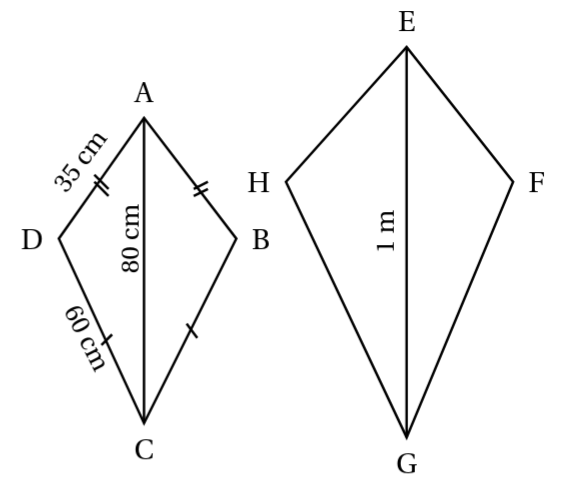
\includegraphics[width=.9\linewidth]{Images/Évaluation 2 - ex DNB.png}

                {\small \emph{Le schéma n’est pas à l’échelle.}}
            \end{center}
        \end{multicols}

    \end{exercice}
    \newpage

    Nom, prénom et classe : \ligne

    \vspace{.5cm}

    \begin{exercice}
        \brm{10}
        \begin{multicols}{2}
            \begin{itemize}[itemsep=10pt]
                \item $0,293 \times 10^3$: \ligne
                \item $737 \times 10^{-1}$: \ligne
                \item $0,083 \times 10^2$: \ligne
                \item $2 \times 10^1$ : \ligne
                \item $6580 \times 10^{-2}$ : \ligne
                \item $\dfrac{4}{7} + \dfrac{1}{7}$: \ligne
                \item $\dfrac{11}{2} \times \dfrac{7}{9}$: \ligne
                \item $\dfrac{7}{5} \div \dfrac{4}{3}$: \ligne
                \item $\dfrac{5}{3} - \dfrac{2}{3}$: \ligne
                \item $3 \times \dfrac{2}{5}$: \ligne
                \item médiane de $9 \,\,;\,\, 8 \,\,;\,\, 15 \,\,;\,\, 6$: \ligne
                \item médiane de $8 \,\,;\,\, 15 \,\,;\,\, 11$: \ligne
                \item moyenne de $6 \,\,;\,\,9\,\,;\,\,15$: \ligne
                \item étendue de $12\,\,;\,\,6\,\,;\,\,8$: \ligne
                \item étendue de $8\,\,;\,\, 13\,\,;\,\, 5\,\,;\,\, 3\,\,;\,\, 9\,\,;\,\,11$: \ligne
                \item écriture réduite de $3 \times (2x+5)$: \ligne
                \item écriture réduite de $m \times (2m - 3)$: \ligne
                \item écriture réduite de $-2 \times (5-y)$: \ligne
                \item écriture réduite de $5+(3x-2)$: \ligne
                \item écriture réduite de $10t - (-3t - 2)$: \ligne
            \end{itemize}
        \end{multicols}
    \end{exercice}
\end{Maquette}


\end{document}